\documentclass[
	letterpaper, % Paper size, specify a4paper (A4) or letterpaper (US letter)
	10pt, % Default font size, specify 10pt, 11pt or 12pt
]{CSUniSchoolLabReport}

%----------------------------------------------------------------------------------------
%	REPORT INFORMATION
%----------------------------------------------------------------------------------------

\title{Operational Amplifiers \\ Circuits \& Signals \\ EECE2150} % Report title

\author{Michael \textsc{Brodskiy}}

\date{February 16, 2023} % Date of the report

%----------------------------------------------------------------------------------------


\begin{document}

\maketitle % Insert the title, author and date using the information specified above

\begin{center}
	\begin{tabular}{l r}
		Date Performed: & February 13, 2023 \\ % Date the experiment was performed
        Partner: & Juan \textsc{Zapata} \\ % Partner names
		Instructor: & Professor \textsc{Sun} % Instructor/supervisor
	\end{tabular}
\end{center}

\setcounter{section}{-1}

\section{Introduction}

The purpose of this laboratory experimentation is to familiarize oneself with the concept of operational amplifiers, as well as supporting circuit construction. By applying the idea of operational amplifiers in real-world scenarios, a more thorough understanding is developed.

\section{Building and Testing}

\begin{figure}[H]
  \centering
  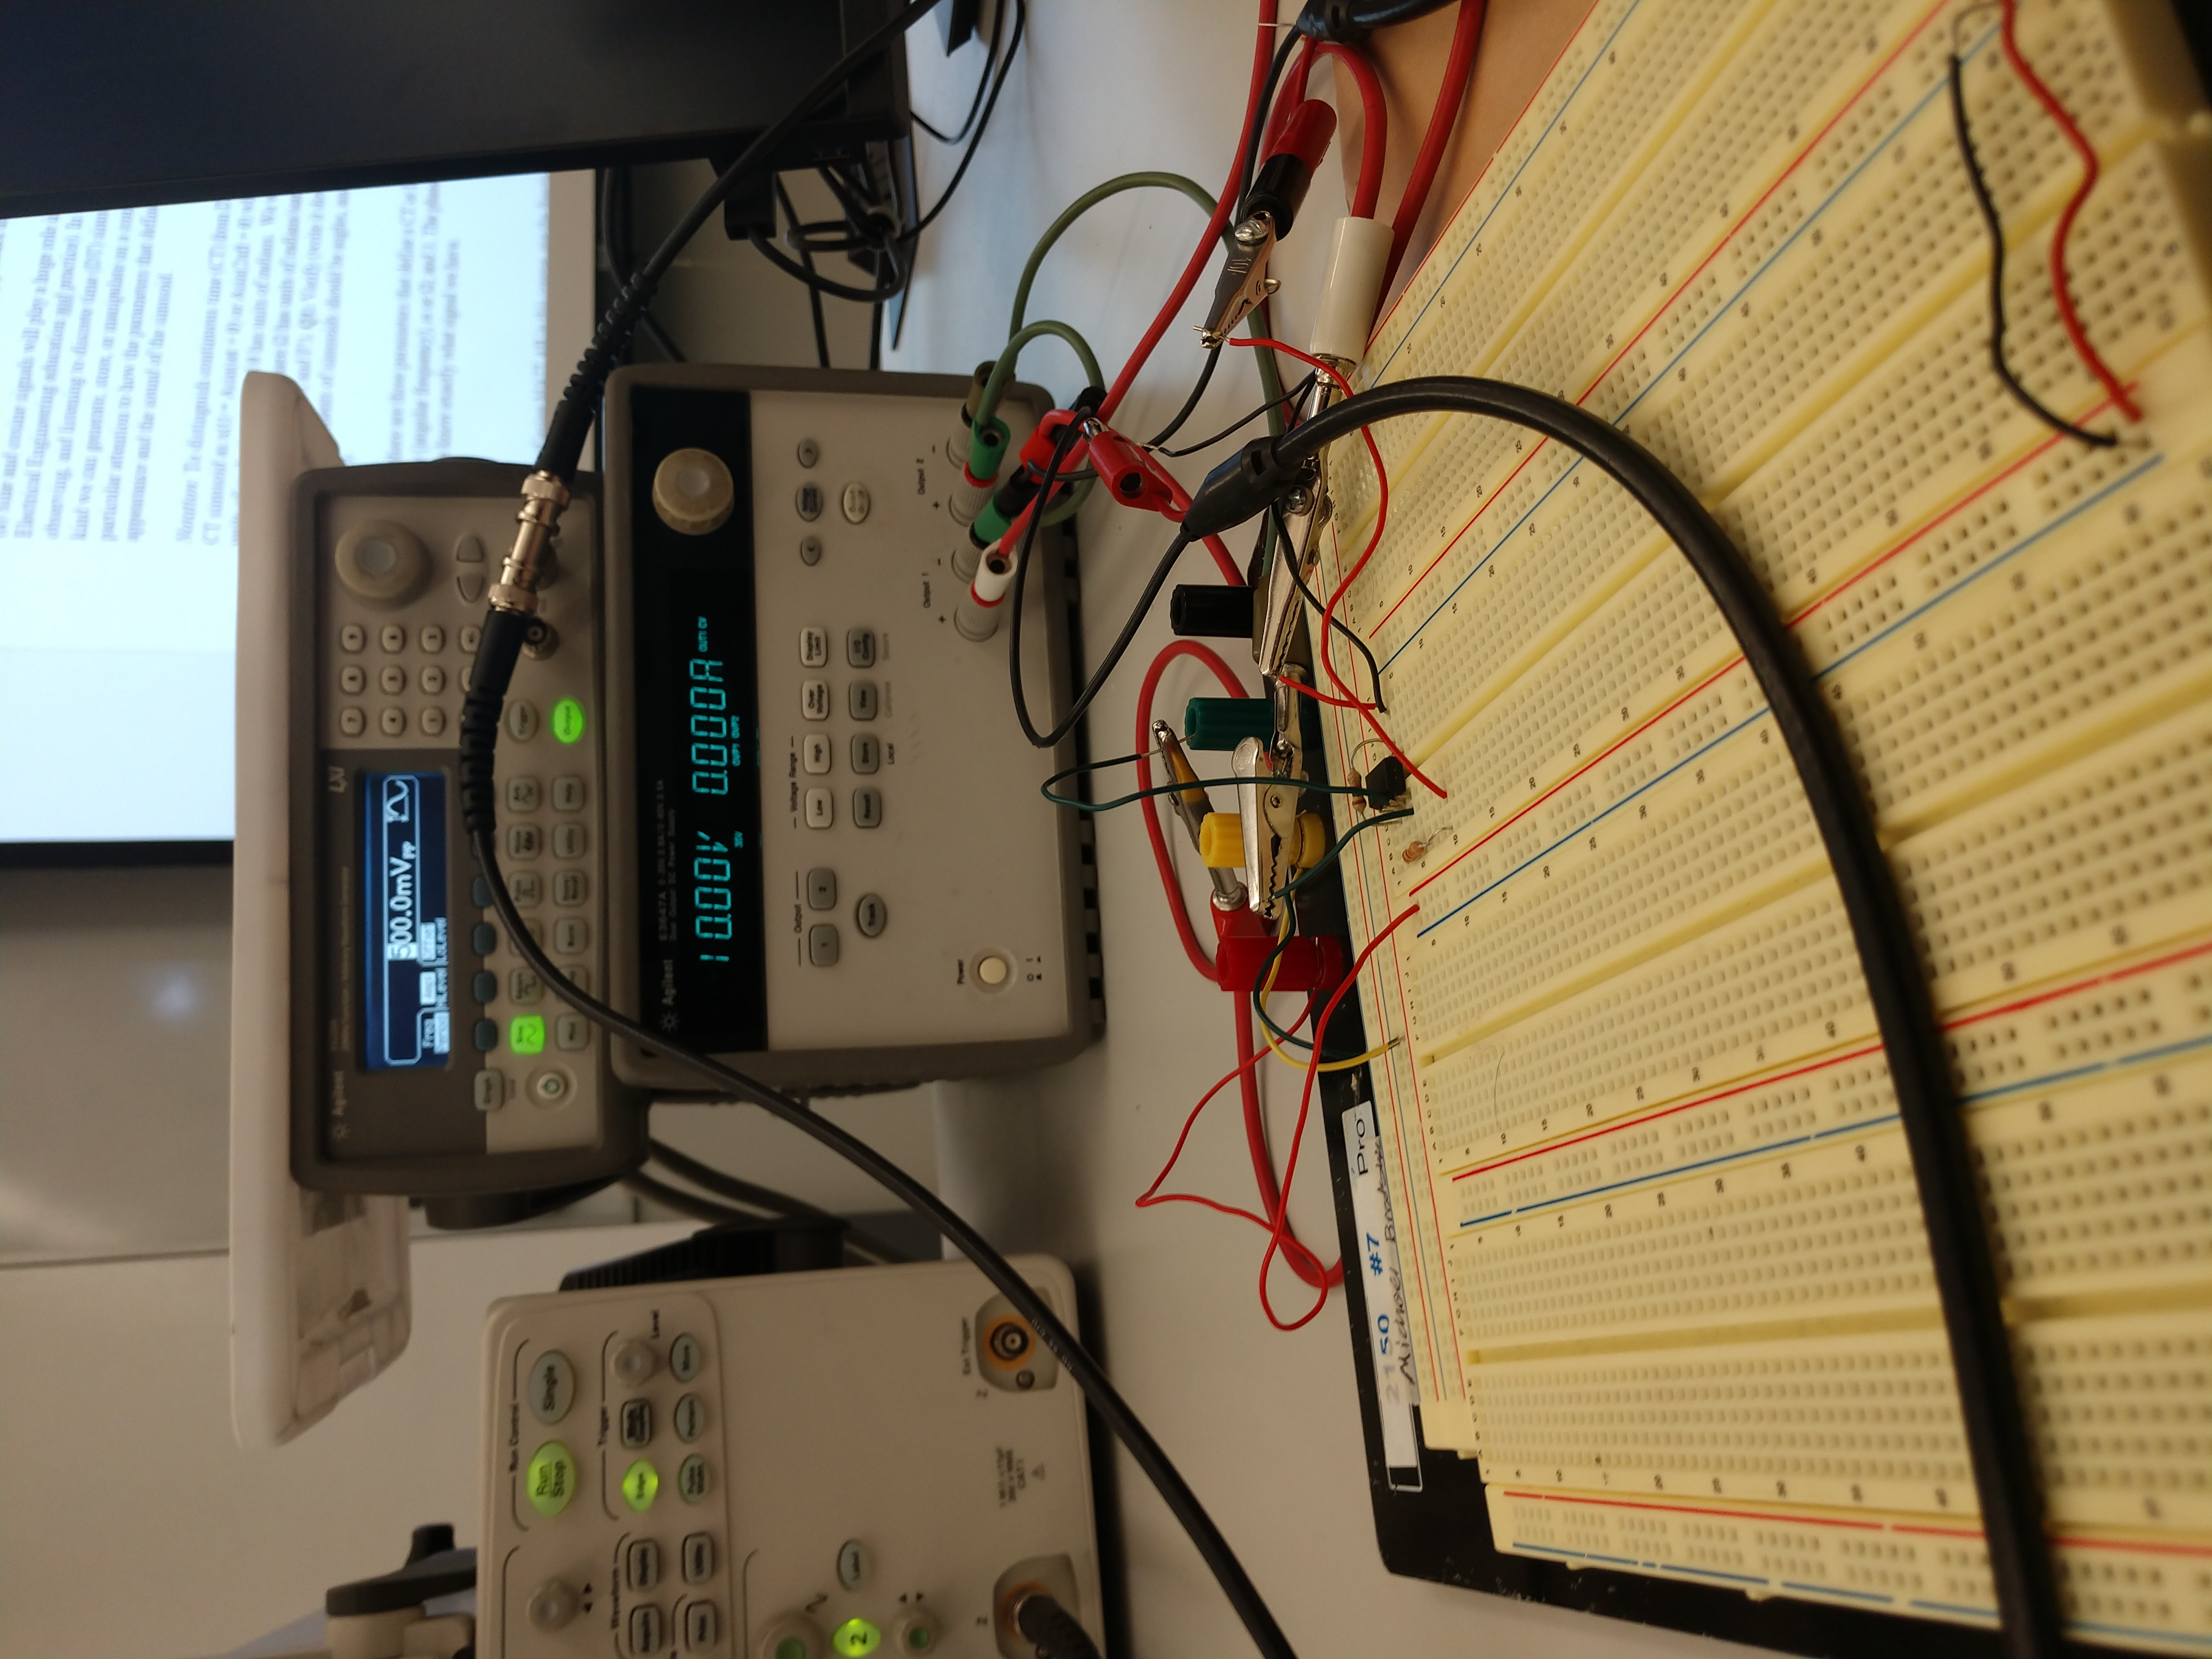
\includegraphics[width=.9\textwidth,angle=270]{Figures/L6Circ}
  \caption{Operational Amplifier Circuit}
  \label{fig:1}
\end{figure}

\subsection{Q1} According to the oscilloscope readings, the gain of the system is approximately $V_o/V_{in}=\mp10/\pm1=-10$

\subsection{Q2} This does agree with the predicted value, as it should be nearly 10 due to the ratio of the feedback resistor to the initial resistor.

\subsection{Q3} It is evident that the gain is negative because the output voltage is a sine wave mirrored about the $x$-axis, as shown in Figure \ref{fig:2}. Thus, due to the phase difference, it is the negative equivalent of the input voltage.

\begin{figure}[H]
  \centering
  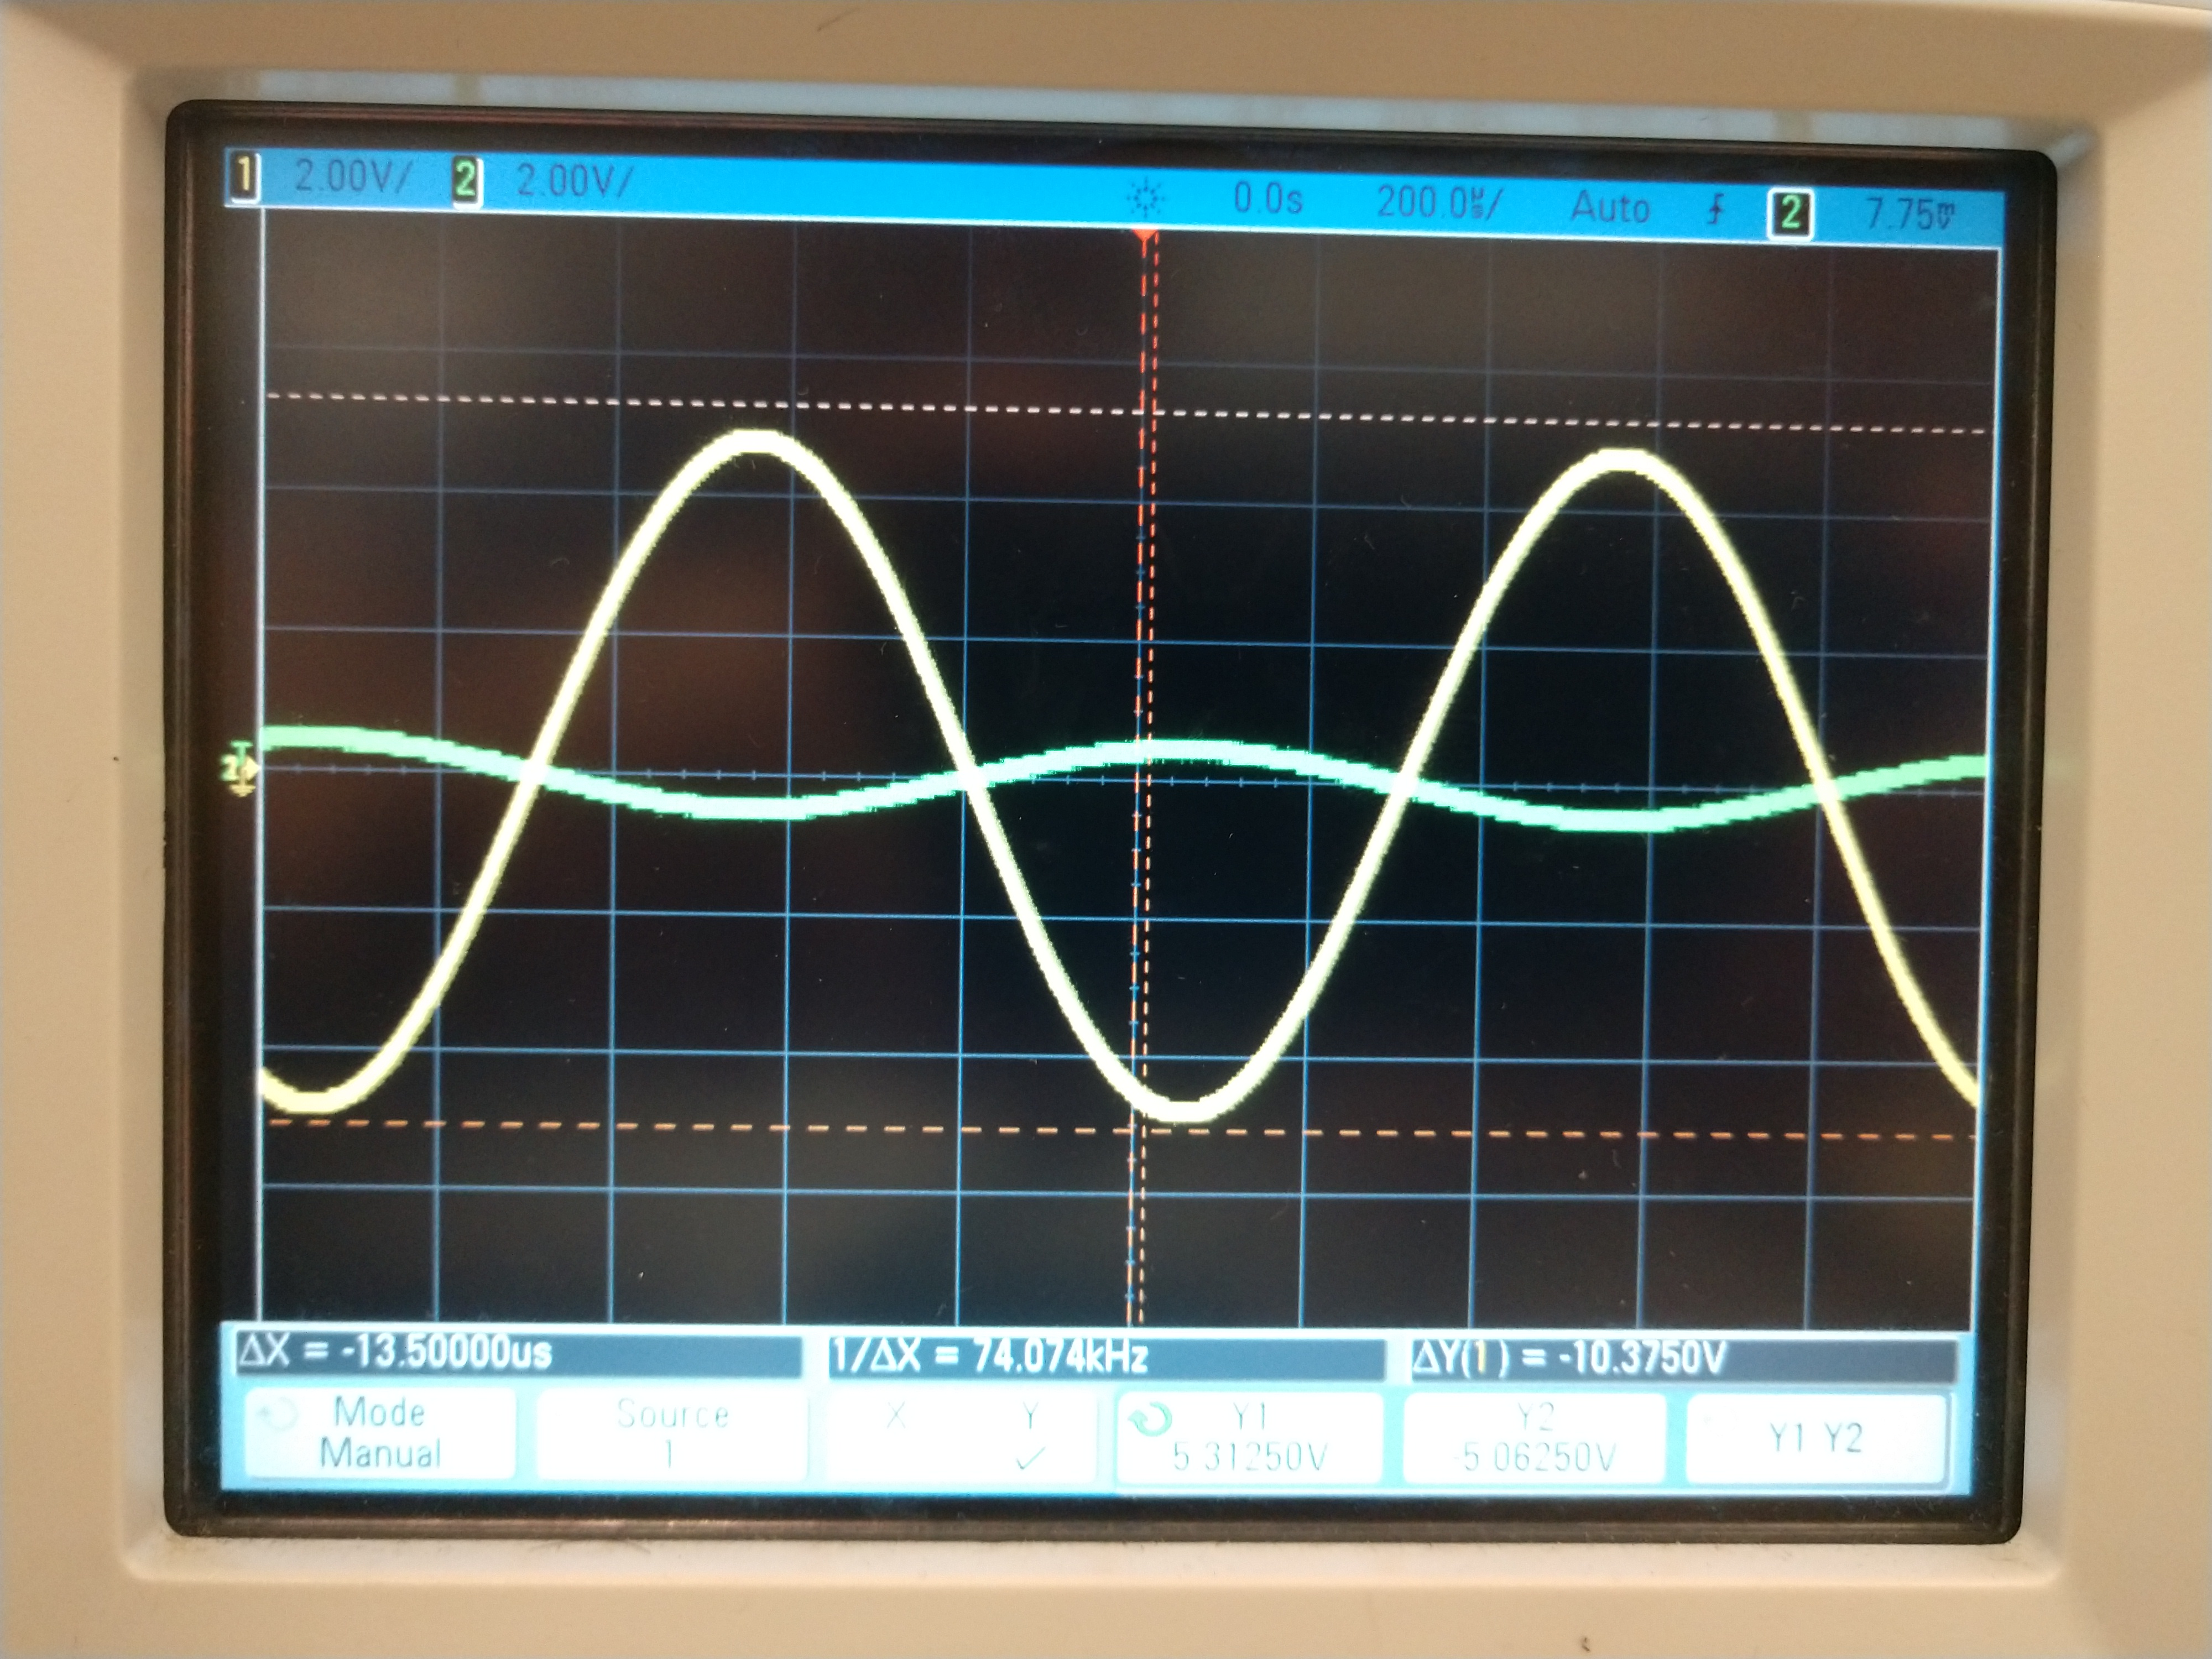
\includegraphics[width=.9\textwidth]{L6OSC}
  \caption{Oscilloscope Reading\footnote{The green wave indicates the input voltage, while the yellow wave indicates the output voltage.}}
  \label{fig:2}
\end{figure}

\subsection{Q4} Upon increasing the peak-to-peak voltage, the amplitude of both waves increased. The input voltage now had an amplitude of $1.2[\si{\volt}]$, and the second wave had an amplitude of $-10(1.2)=-12[\si{\volt}]$. One thing to note, however, is that the output voltage wave hit the oscilloscope display threshold, effectively limiting it to only $10[\si{\volt}]$ peaks.

\subsection{Q5} This was accomplished by constructing a simple voltage divider to achieve the desired voltage output. Two resistors, one of $9[\si{\kilo\ohm}]$ and another of $1[\si{\kilo\ohm}]$ were daisy-chained together and placed in the circuit (connected to the DC generator) as if it was a single resistor with $1[\si{\volt}]$ across it. 

\subsection{Q6} The circuit output is shifted up by $1[\si{\volt}]$, as all alternating current values are increased by the $1[\si{\volt}]$ constant direct current voltage.

\subsection{Q7} This is the expected result, as, due to the constant value of the DC output, as compared to the AC, 1 volt would be added to the AC value at every point.

\section{Conclusion}

Overall, this laboratory experiment allowed us to develop a fully-working operational amplifier circuit; in doing so, the concepts became much clearer than they were in in-class presentations. As such, a solid foundation for this concept was fabricated.

\end{document}
